\documentclass[10pt,twocolumn,a4paper]{ctexart}
\usepackage[margin=1.7cm,columnsep=0.65cm]{geometry}
\usepackage{amsmath,amssymb,bm}
\usepackage{booktabs}
\usepackage{graphicx}
\usepackage{microtype}
\usepackage{natbib}
\usepackage{xcolor}
\usepackage{hyperref}
\usepackage{enumitem}
\usepackage{fancyhdr}
\usepackage{float}

\graphicspath{{../../artifacts/figures/}}
\renewcommand{\topfraction}{0.9}\renewcommand{\dbltopfraction}{0.9}
\renewcommand{\textfraction}{0.07}\renewcommand{\floatpagefraction}{0.75}
\renewcommand{\dblfloatpagefraction}{0.75}\setcounter{topnumber}{3}\setcounter{dbltopnumber}{2}
\setlength{\parindent}{2em}
\setlist{nosep,leftmargin=*}
\hypersetup{colorlinks=true,linkcolor=blue!55!black,
  citecolor=green!45!black,urlcolor=blue!65!black}
\pagestyle{fancy}
\fancyhf{}
\fancyhead[L]{CS224R 2025 Homework 4}
\fancyhead[R]{ShaneLiu04}
\fancyfoot[C]{\thepage}

\newcommand{\figmaybe}[2]{%
  \IfFileExists{../../artifacts/figures/#1.png}{%
    \includegraphics[width=\linewidth]{#1}}{%
    \fbox{\parbox[c][3.2cm][c]{\linewidth}{\centering\small #2}}}}

\title{\vspace{-1.2em}\textbf{稀疏奖励下的目标重标注与解耦元探索：\\
HER、RL$^2$ 与 DREAM}}
\author{ShaneLiu04\\
\small\url{https://github.com/ShaneLiu04}}
\date{}

\begin{document}
\maketitle
\thispagestyle{fancy}

\begin{abstract}
本文完成 CS224R 2025 Homework 4 的两部分。第一部分在 goal-conditioned DQN 上实现
Hindsight Experience Replay（HER）的 \texttt{final}、\texttt{future}、\texttt{random}
三种重标注，并在 bit flipping（$n=6,15,25$）与 MuJoCo Sawyer Reach 上与无重标注的
基线比较。$15$ 位与 $25$ 位任务上，无 HER 的成功率在全部 $5$ 个种子上都是 $0$，三种
HER 都是 $1.0$；Sawyer 的稠密奖励让基线也能达到 $0.55\pm0.11$，HER 提到
$0.95$--$0.99$。第二部分实现 DREAM 的解码器损失与信息增益奖励。网格公交任务上，
DREAM 的元测试回报为 $0.696\pm0.007$（$5$ 个种子），等于我们推导的最优值 $0.7$；
RL$^2$ 为 $0.143\pm0.073$，接近直接步行的 $0.1$。额外实验包括重标注比例 $k$ 的扫描、
Sawyer 上的 \texttt{future}/\texttt{random}，以及去掉每步探索惩罚 $c$ 的 DREAM 消融。
\end{abstract}

\textbf{关键词：}Goal-Conditioned RL；HER；Sparse Reward；Meta-RL；RL$^2$；DREAM

\section{问题}
Goal-conditioned RL 在每个 episode 采样目标 $g$，奖励 $r(s,a,g)$ 只在到达 $g$ 时
不同于失败\citep{kaelbling1993goals,schaul2015uvfa}。bit flipping 的状态与目标都是
$n$ 位二进制串，动作翻转一位，奖励在 $s=g$ 时为 $0$、否则为 $-1$，episode 长度为 $n$。
随机初始化的 Q 网络几乎不会碰到 $r=0$，DQN 的所有 TD 目标都是常数，学不到动作偏好
\citep{andrychowicz2017her}。Sawyer Reach 是机械臂末端在平面内到达目标点，动作离散
为四个方向，奖励为 $-\lVert x-g\rVert$\citep{nair2018rig,todorov2012mujoco}。

Meta-RL 部分是 $5\times5$ 网格：智能体从中心出发，目标是四个角之一；中心四周有四个
公交站，乘车会被传送到某个角，$24$ 个任务只在公交目的地的排列上不同；右侧中间的
地图格子会显示当前任务 ID\citep{liu2021dream}。每次元测试有一个探索 episode 和一个
利用 episode，只计利用 episode 的回报。

\section{方法}
\subsection{Goal-conditioned DQN 与 HER}
Q 网络输入 $[s;g]$，输出各动作的 Q 值；采样时取 greedy 动作。DQN 每个 epoch 采集
$16$ 条轨迹，做 $40$ 次批大小 $128$ 的更新，$\gamma=0.98$，目标网络每个 epoch 同步一次，
TD 目标截断到 $[-1/(1-\gamma),0]$\citep{mnih2015dqn}。

\texttt{update\_replay\_buffer} 先写入原转移 $(s_t,a_t,r_t,s_{t+1},g)$，再为每个时间步
生成 $k=4$ 条重标注转移（\texttt{final} 只生成一条）：
\begin{itemize}
\item \texttt{final}：$g'=s_{T}$，即最后一个 \texttt{next\_state}；
\item \texttt{future}：$g'=s_{j+1}$，$j\sim\mathcal{U}\{t,\ldots,T-1\}$；
\item \texttt{random}：$g'=s_{j+1}$，$j\sim\mathcal{U}\{0,\ldots,T-1\}$。
\end{itemize}
奖励由环境的奖励函数 $r(s_{t+1},g')$ 重算，数组全部 \texttt{copy()}。我们为
\texttt{main.py} 增加了 \texttt{--num\_relabeled}，用于扫描 $k$。

\subsection{DREAM}
解码器 $q_\omega(z\mid\tau)=\mathcal{N}(g_\omega(\tau),I)$，最大化
$\mathbb{E}[\log q_\omega(z\mid\tau^{\exp})]$ 等价于最小化
\begin{equation}
\mathcal{L}_{\mathrm{dec}}=\mathbb{E}\bigl\lVert g_\omega(\tau^{\exp})-\mathrm{sg}(z)\bigr\rVert_2^2 .
\end{equation}
实现上对 \texttt{all\_decoder\_embeddings} 的每个前缀计算与 \texttt{stop\_gradient}($z$)
的平方距离，沿嵌入维求和、沿时间与 batch 取平均。探索奖励是相邻前缀的信息增益
\begin{equation}
r_t^{\exp}=\lVert g(\tau_{:t})-z\rVert^2-\lVert g(\tau_{:t+1})-z\rVert^2 ,
\end{equation}
即距离序列的差分 \texttt{distances[:, :-1] - distances[:, 1:]}。starter 再从每步奖励中
减去常数 $c=0.1$（论文式 (5)），使探索策略在不再获得信息时倾向于结束 episode
\citep{liu2021dream}。编码器 $F_\psi(z\mid\mu)$ 另有信息瓶颈项
$\max(\lVert z\rVert^2,10)$，配合编码噪声限制 $z$ 携带的信息量\citep{alemi2017vib}。

\subsection{实验设置}
bit flipping 按作业的 epoch 数（$250/500/1000$）运行，$6$ 位 $3$ 个种子，$15$、$25$ 位
$5$ 个种子；Sawyer 运行 $1000$ 个 epoch、$5$ 个种子，四种重标注都跑。$k$ 扫描在 $15$ 位
\texttt{future} 上取 $k\in\{1,2,8\}$，各 $3$ 个种子，$k=4$ 复用主实验。DREAM 与 RL$^2$
各 $5$ 个种子，$c=0$ 的 DREAM $3$ 个种子。最终成功率取每个种子最后 $10$（bit
flipping）或 $20$（Sawyer）个记录点的均值，再报告跨种子的均值与标准差。全部运行在
CPU 上并行完成，曲线由 TensorBoard 事件文件导出为 CSV 后统一绘制。

\section{Problem 0：网格任务的最优回报}
中心 $(2,2)$ 到任一角的曼哈顿距离为 $4$。
\begin{enumerate}[label=(\alph*)]
\item 直接步行：前三步各得 $-0.3$，第四步到达得 $+1$，回报 $1-0.9=0.1$。
\item 已知公交目的地时，走一步到通往目标角的公交站（四个站都与中心相邻），再乘车
直达目标：$-0.3+1=0.7$，这是单个利用 episode 的最优回报。
\item 地图在 $(4,2)$，距中心两步。最快的探索是直接走到地图格子读出任务 ID，
共 $2$ 步；之后的动作不再提供信息。
\item 探索 episode 的回报不计入目标，因此元 RL 智能体的最优利用回报就是 $0.7$。
\end{enumerate}

\section{HER on bit flipping}
\begin{figure*}[!t]
\centering
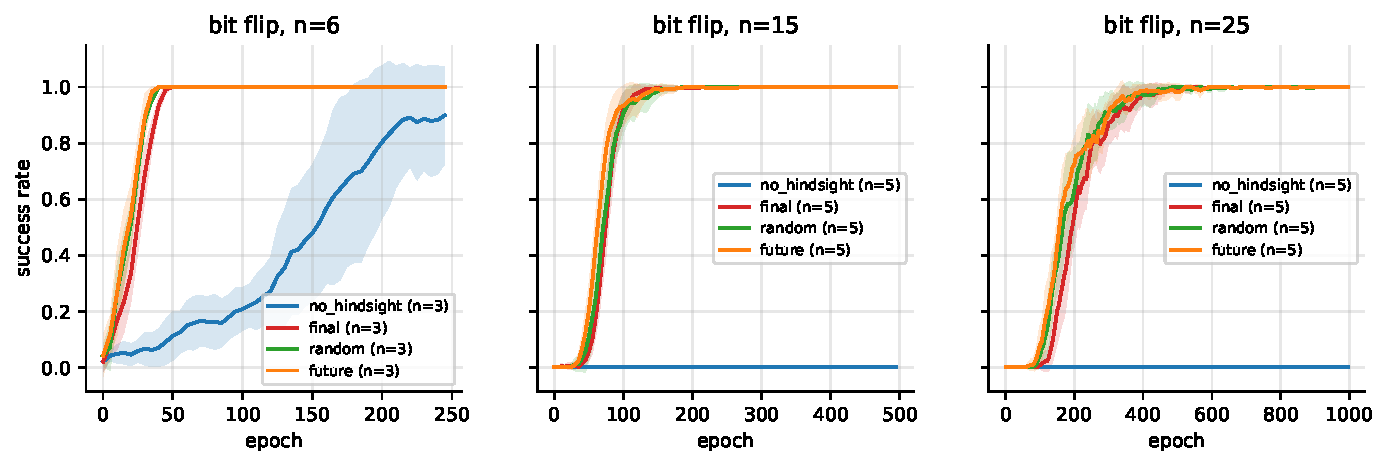
\includegraphics[width=0.95\linewidth]{hw4_fig1_bitflip_success}
\caption{bit flipping 的评估成功率（均值 $\pm$ 标准差，阴影）。$n=6$ 时无 HER 也能学会；
$n=15,25$ 时无 HER 始终为 $0$，三种 HER 都收敛到 $1$。}
\label{fig:bitflip}
\end{figure*}

\begin{table}[H]
\centering
\caption{bit flipping 的最终成功率与首次达到 $0.9$ 的 epoch（滑动平均）。}
\label{tab:bitflip}
\small
\begin{tabular}{lccc}
\toprule
 & $n=6$ & $n=15$ & $n=25$ \\
\midrule
no hindsight & $0.90\pm0.14$ / 245 & $0.00$ / -- & $0.00$ / -- \\
final & $1.00$ / 40 & $1.00$ / 100 & $1.00$ / 320 \\
random & $1.00$ / 35 & $1.00$ / 100 & $1.00$ / 290 \\
future & $1.00$ / 35 & $1.00$ / 90 & $1.00$ / 300 \\
\bottomrule
\end{tabular}
\end{table}

图~\ref{fig:bitflip} 与表~\ref{tab:bitflip} 对应作业的 (a)--(d)。$n=6$ 时状态空间只有
$64$ 个目标，随机初始化的 greedy 策略偶尔能在 $6$ 步内命中，无 HER 的 DQN 能学，
但三个种子里有一个只到 $0.69$，达到 $0.9$ 要到第 $245$ 个 epoch；HER 在 $35$--$40$ 个
epoch 内就达到 $0.9$。$n=15$ 与 $n=25$ 时，随机命中的概率约为 $2^{-n}$ 量级，回放缓冲区里
没有任何 $r=0$ 的转移，Q 函数没有可区分动作的信号，无 HER 的成功率在全部种子上都是
$0$。HER 把每条失败轨迹变成若干条到达“它自己经过的状态”的成功示范，正样本比例
与 $n$ 无关，因此 $25$ 位任务也能学会，只是收敛所需的 epoch 随 $n$ 增长（$90$--$100$ 到
$290$--$320$）：目标空间更大，Q 网络需要更多样本才能泛化到任务目标。

三种重标注最终都达到 $1.0$。\texttt{future} 在 $15$ 位上略快（$90$ 对 $100$），
\texttt{random} 在 $25$ 位上略快（$290$ 对 $300$、$320$），差距都在一个记录间隔左右。
bit flipping 是可逆的：任何经过的状态，无论在 $t$ 之前还是之后，都能从 $s_t$ 翻回去，
所以 \texttt{random} 不会产生不可达目标；而 \texttt{final} 虽然每条轨迹只给一个新目标，
在短 episode（长度为 $n$）上已经足够。在不可逆或长 horizon 的环境里，\texttt{future}
的可达性保证才会显出优势\citep{andrychowicz2017her,plappert2018multigoal}。

\begin{figure}[H]
\centering
\figmaybe{hw4_fig2_bitflip_heatmap}{heatmap}
\caption{最终成功率热图：行为位数，列为重标注策略。}
\label{fig:heat}
\end{figure}

\paragraph{重标注比例 $k$。}图~\ref{fig:k} 在 $15$ 位 \texttt{future} 上比较 $k=1,2,4,8$。
四条曲线几乎重合，首次达到 $0.9$ 的 epoch 为 $90$--$95$。在这个任务上，只要有重标注，
正样本就已不再稀缺；瓶颈转为 Q 网络对新目标的泛化与每个 epoch 固定的 $40$ 次更新，
增加 $k$ 并不能加快学习。

\begin{figure}[H]
\centering
\figmaybe{hw4_fig5_her_k}{her k}
\caption{$15$ 位 \texttt{future} HER 中每条转移的重标注数 $k$。}
\label{fig:k}
\end{figure}

\section{HER on Sawyer Reach}
\begin{figure*}[!t]
\centering
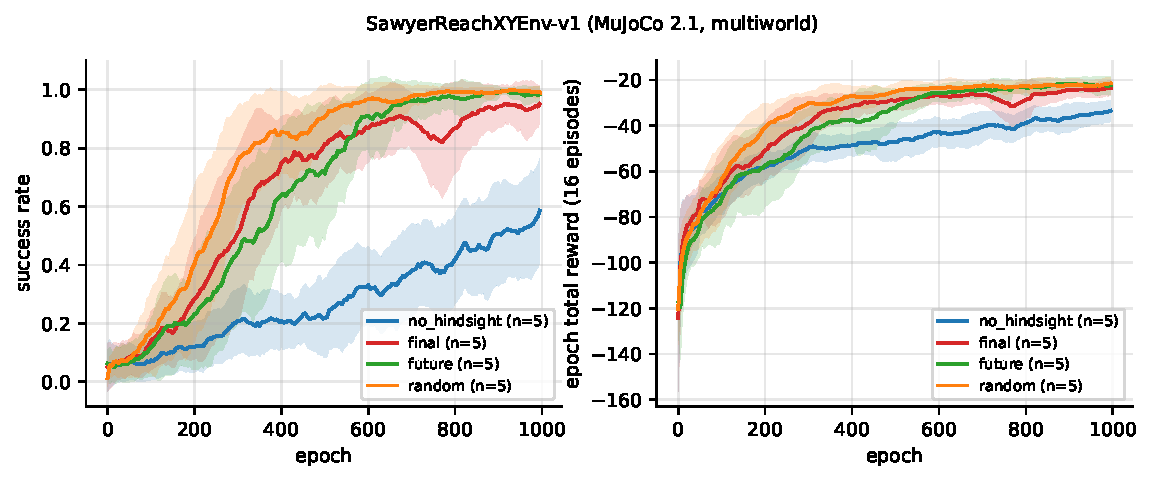
\includegraphics[width=0.85\linewidth]{hw4_fig3_sawyer}
\caption{Sawyer Reach 的成功率与每个 epoch 的总奖励（$5$ 个种子）。}
\label{fig:sawyer}
\end{figure*}

图~\ref{fig:sawyer} 中，无 HER 的成功率在 $1000$ 个 epoch 后为 $0.55\pm0.11$，仍在缓慢上升；
\texttt{final} 为 $0.95\pm0.05$，\texttt{future} 为 $0.99\pm0.01$，\texttt{random} 为
$0.99\pm0.01$。滑动成功率首次达到 $0.8$ 的 epoch 分别为 \texttt{random} $335$、
\texttt{final} $495$、\texttt{future} $550$，无 HER 未达到。

与 bit flipping 的差别在奖励结构。Sawyer 的奖励 $-\lVert x-g\rVert$ 是稠密的：
即使从未到达目标，每一步也告诉智能体离目标多远，DQN 能学到“朝目标移动”，所以基线
不是 $0$。HER 在这里的作用是让每条轨迹在更多目标上提供监督，提高样本效率与末端精度，
而不是像 bit flipping 那样从 $0$ 到 $1$。总奖励曲线也反映这一点：四种方法的回报差距
远小于成功率差距，因为成功只看最后是否落入阈值，而奖励在接近目标时已经很高。
\texttt{final} 在第 $700$--$800$ 个 epoch 有一次明显下滑，标准差也最大；只用末状态作目标，
新目标集中在策略常去的区域，覆盖不如另外两种均匀。

\section{Meta-RL}
\begin{figure*}[!t]
\centering
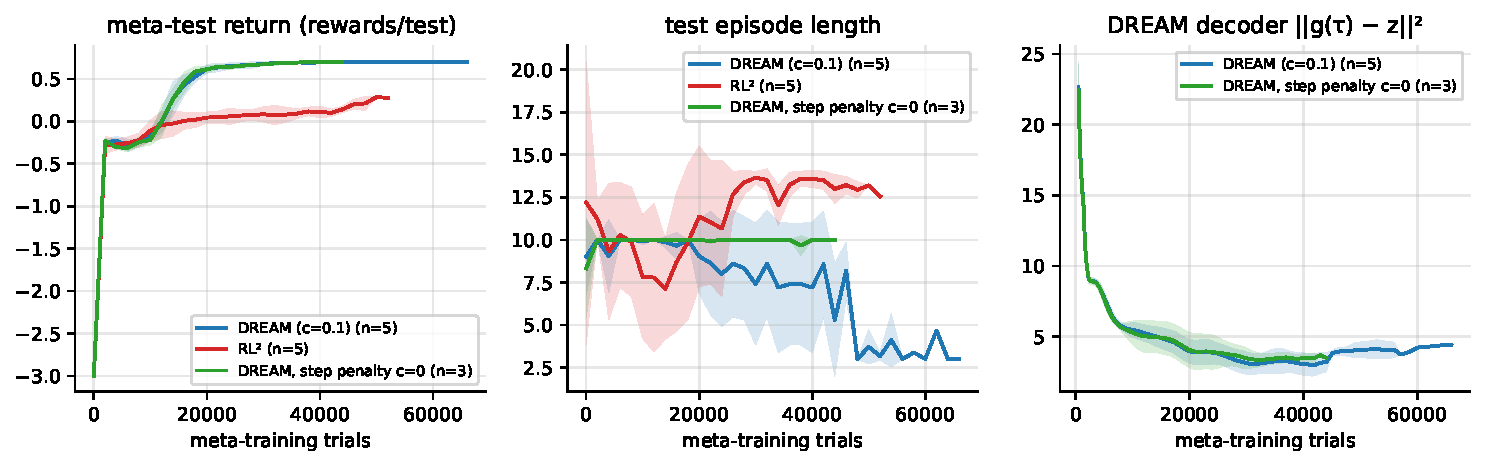
\includegraphics[width=0.95\linewidth]{hw4_fig4_meta_rl}
\caption{左：元测试利用回报。中：DREAM 为探索 episode 长度，RL$^2$ 为测试 episode 长度
（RL$^2$ 的探索与利用在同一条轨迹中）。右：DREAM 的解码误差。}
\label{fig:meta}
\end{figure*}

\subsection{RL$^2$}
RL$^2$ 训练约 $5\times10^4$ 个元训练 trial 后，最后三次评估的元测试回报为
$0.143\pm0.073$（$5$ 个种子：$0.07,0.16,0.10,0.28,0.12$），保留一位小数约为 $0.1$，
与直接步行的回报一致，远低于最优的 $0.7$。图~\ref{fig:frames} 最下一行是一个种子在
$52\,000$ 个 trial 时的轨迹：智能体有时会走到地图附近，但利用阶段并没有稳定地选择
通往目标的公交，大多数情况下仍在步行。RL$^2$ 的测试 episode 长度维持在 $13$ 步左右，
说明探索段被用来游走，而不是用最短的 $2$ 步读取地图。原因在于端到端优化的耦合：
只有当利用策略已经会使用地图信息时，走到地图才有回报；而利用策略只有在探索收集到
信息时才能学会使用它。训练早期两者都差，探索得不到梯度信号，策略停在“忽略任务信息、
直接步行”的局部最优\citep{duan2016rl2,liu2021dream}。少数种子在训练后期回报开始上升
（$0.28$），说明这一局部最优可以逃离，但需要远多于 DREAM 的样本。

\subsection{DREAM}
DREAM 的回报在约 $1.5\times10^4$ 个 trial 后开始与 RL$^2$ 分离，约 $3\times10^4$ 个 trial
后稳定在 $0.7$，最后三次评估为 $0.696\pm0.007$，$5$ 个种子里有 $4$ 个恰为 $0.70$。这达到了
Problem 0 推导的最优值，符合预期：DREAM 用问题 ID 训练的编码器为探索提供了稠密的
信息增益奖励，打破了探索与利用的鸡生蛋循环。解码误差从约 $23$ 迅速降到 $4$ 左右，
不再归零，因为 $z$ 带有编码器的噪声，且解码器在第一步之前无法知道任务。

图~\ref{fig:frames} 第一行是 DREAM 在 $56\,000$ 个 trial 时的行为。探索 episode 中，
智能体从中心向右走两格到达地图（黑色格子）后停止，episode 长度为 $3$ 步，正是
Problem 0(c) 的最短探索。利用 episode 中，智能体走一步到通往目标角的公交站并乘车，
两步到达目标，回报 $0.7$。

\begin{figure*}[!t]
\centering
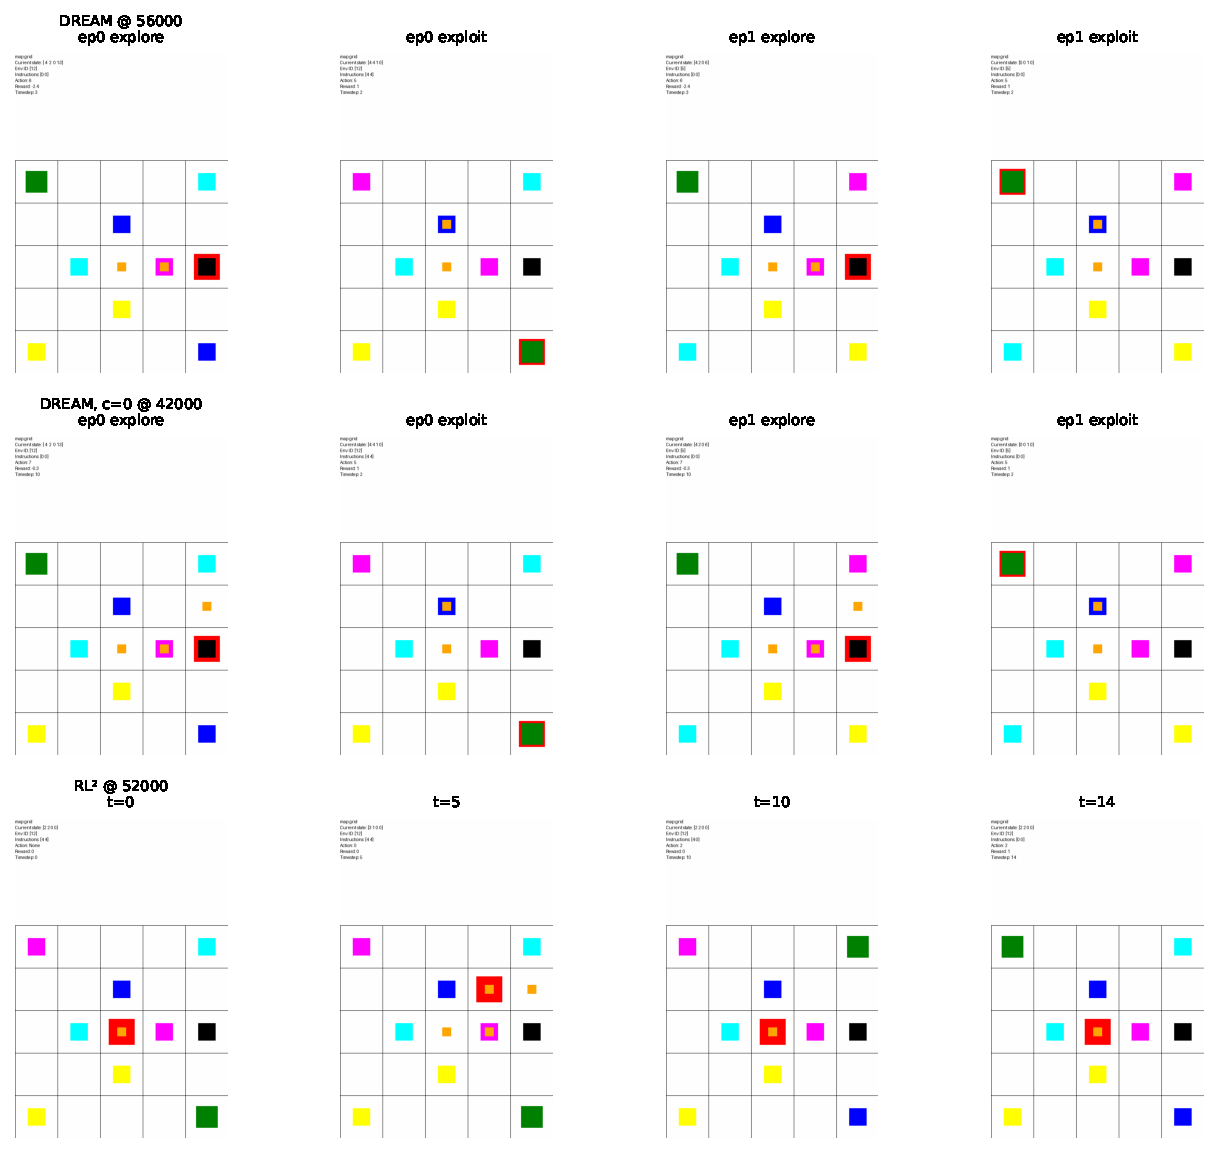
\includegraphics[width=0.9\linewidth]{hw4_fig6_meta_frames}
\caption{元测试 rollout 的最后一帧。橙色小方块为本 episode 访问过的格子，黑色为地图，
绿色为目标，红色为智能体。前两行为 DREAM 及其 $c=0$ 消融的两个元测试 episode，
最后一行为 RL$^2$ 同一条轨迹的四个时刻。}
\label{fig:frames}
\end{figure*}

\subsection{每步探索惩罚的消融}
把探索奖励中的常数 $c$ 设为 $0$ 后，三个种子的元测试回报同样是 $0.70$，收敛速度与默认
DREAM 几乎相同（图~\ref{fig:meta} 左）。差别出现在探索行为上：$c=0$ 的探索 episode
长度始终在 $10$ 步左右（$9.9\pm0.2$），即用满上限；默认 $c=0.1$ 的五个种子最终为
$8.4,10,3.6,10,3.0$，其中两个种子学会了“读完地图就结束”的 $3$ 步探索。
图~\ref{fig:frames} 第二行显示，$c=0$ 时智能体同样先到地图，但之后继续游走。
走到地图那一步之后，解码器已经能恢复 $z$，后续每步的信息增益约为 $0$；$c=0$ 时这些步
没有代价，探索策略没有理由结束 episode，$c>0$ 时它们的回报为 $-c$，最优行为是立即结束。
由于本设定只计利用回报，探索长度不影响最终分数，$c$ 的作用只体现在探索效率上；
在探索步数本身有成本，或者需要多次探索 episode 的设定里，这一项才会改变回报
\citep{liu2021dream}。另有三个默认种子的探索仍接近 $10$ 步，说明 $c=0.1$ 带来的信号
较弱，“提前结束”需要额外的训练才能被发现。

\section{结论}
HER 的收益随奖励稀疏程度增长：bit flipping 中它是能否学会的决定因素，Sawyer 的稠密
奖励下它把成功率从 $0.55$ 提到 $0.95$ 以上。在可逆的 bit flipping 上，三种重标注策略
与 $k\in\{1,2,4,8\}$ 的差别都很小。Meta-RL 中，端到端的 RL$^2$ 停在步行回报 $0.1$
附近，DREAM 借助问题 ID 解耦探索与利用，达到最优的 $0.7$；每步探索惩罚 $c$ 在本任务中
不改变最终回报，但让部分种子学到最短的探索轨迹。

\clearpage
\bibliographystyle{plainnat}
\bibliography{../references}

\end{document}
